\documentclass[12pt]{article}
\usepackage[utf8]{inputenc} % Pacote para acentuação gráfica
%\usepackage[T1]{fontenc}
\usepackage[brazil]{babel} % nomes das estruturas em pt-br
%\usepackage{hyperref}
\usepackage{indentfirst} % indenta primeiro paragráfo após título
\usepackage{setspace} % pacote para alterar espaçamento entre linhas
%\setlength{\parindent}{1cm} % define o tamanho da indentação
%\setlength{\parskip}{0.3cm} % define o espaçamento vertical entre parágrafos
\usepackage[top = 2cm, left = 2cm, bottom = 2cm, right = 2cm]{geometry} % define as margens do documento
\usepackage{fancyhdr} % pacote para numeração de páginas
\usepackage{lipsum}  % Pacote para gerar texto de preenchimento
\usepackage{xcolor} % Definindo novas cores
\usepackage{graphicx} % para inserir figuras
\usepackage{float} % Força o posicionamento da figura


\definecolor{verde}{rgb}{0.25,0.5,0.35}
\definecolor{jpurple}{rgb}{0.5,0,0.35}
% Configurando layout para mostrar codigos Java
\usepackage{listings}
\lstset{
	language=Python,
	basicstyle=\ttfamily\small,
	keywordstyle=\color{jpurple}\bfseries,
	stringstyle=\color{red},
	commentstyle=\color{verde},
	morecomment=[s][\color{blue}]{/**}{*/},
	extendedchars=true,
	showspaces=false,
	showstringspaces=false,
	numbers=left,
	numberstyle=\tiny,
	breaklines=true,
	backgroundcolor=\color{cyan!10},
	breakautoindent=true,
	captionpos=b,
	xleftmargin=0pt,
	tabsize=4
}
\pagestyle{empty}

\begin{document}
	
\title{\textbf{{\Huge Notas em Computação Quântica}}} % Título
\author{\textbf{{\Large Ricardo Alvarenga}}} % Autor
\date{\textbf{{\Large 2024}}} % Data
\maketitle % Criar
\thispagestyle{empty} % oculta número da página
\newpage

\pagestyle{fancy}
\setcounter{page}{1} % reset contador de página
\pagenumbering{Roman}  % Altera número de página para números romanos
\tableofcontents % cria sumário
\newpage

\listoffigures % lista de figuras
\newpage


\pagestyle{fancy}
\fancyfoot[C]{\thepage} % Adiciona o número da página no centro do rodapé
\newpage

\setcounter{page}{1} % reset contador de página
\pagenumbering{arabic}
\pagestyle{fancy}
\fancyfoot[C]{\thepage}

% \twocolumn  % Inicia o ambiente de duas colunas

\section{Álgebra Linear}

\subsection{Vetores}

Vetores são seguimentos orientados (início em 0, 0) que estão sempre no plano cartesiano. Vetores são usados para representar grandezas escalares (massa, pressão, etc.) e grandezas físicas vetoriais (velocidade, força e deslocamento).

\begin{figure}[H]
	\centering
	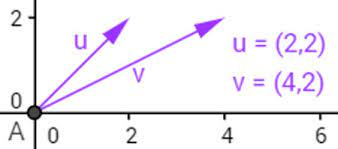
\includegraphics[width=.5\linewidth]{figuras/vetores_01}
	\caption[Vetores \textbf{u} e \textbf{v}]{Exemplos de Vetores, \textbf{u} e \textbf{v}}
	\label{fig:vetores01}
\end{figure}

\subsubsection{Vetores Com Duas Dimensões - R2}

\textbf{x}, \textbf{y} podem assumir qualquer valor \textit{Real}.

\begin{figure}[H]
	\centering
	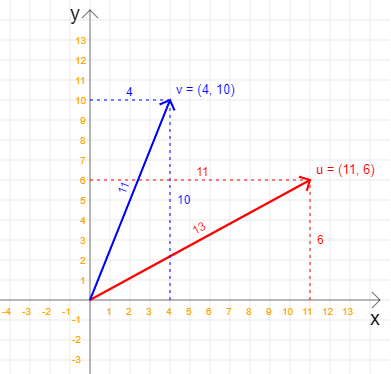
\includegraphics[height=.45\textheight]{figuras/vetores_02}
	\caption[Vetores em R2]{Vetores em R2 (x, y)}
	\label{fig:vetores02}
\end{figure}

\newpage

\subsubsection{Vetores Com Três Dimensões - R3}

\textbf{x}, \textbf{y}, \textbf{z} podem assumir qualquer valor \textit{Real}.

\begin{figure}[H]
	\centering
	\includegraphics[width=0.5\linewidth]{"figuras/vetores R3"}
	\caption[Vetores em R3]{Vetores em R3 (x, y, z)}
	\label{fig:vetores-r3}
\end{figure}

\subsubsection{Vetores Com n Dimensões - Rn}

Os vetores com \textit{n} dimensões são de difícil (ou impossível) representação gráfica.

Um vetor R4 é indicado da seguinte forma: R4(x, y, z, w)

\subsubsection{Tipos de Vetores}
\subsubsection{Igualdade de Vetores}
\subsubsection{Soma e Multiplicação por Coeficiente dos Vetores}
\subsubsection{Produto Escalar dos Vetores (Multiplicação)}
\subsubsection{Módulo de Um Vetor}
\subsubsection{Ângulo de Dois Vetores}
\subsubsection{Paralelismo e Ortogonalidade de Dois Vetores}
\subsubsection{Projeção Ortogonal Entre Dois Vetores}

% \lipsum[1-10]  % Exemplo de texto de preenchimento



	
\end{document}